%%%%%%%%%%%%%%%%%%%%%%%%%%%%%%%%%%%%%%%%%
% baposter Landscape Poster
% LaTeX Template
% Version 1.0 (11/06/13)
%
% baposter Class Created by:
% Brian Amberg (baposter@brian-amberg.de)
%
% This template has been downloaded from:
% http://www.LaTeXTemplates.com
%
% License:
% CC BY-NC-SA 3.0 (http://creativecommons.org/licenses/by-nc-sa/3.0/)
%
%%%%%%%%%%%%%%%%%%%%%%%%%%%%%%%%%%%%%%%%%

%----------------------------------------------------------------------------------------
%	PACKAGES AND OTHER DOCUMENT CONFIGURATIONS
%----------------------------------------------------------------------------------------

\documentclass[landscape,a0paper,fontscale=0.3]{baposter} % Adjust the font scale/size here

\usepackage{graphicx} % Required for including images
\graphicspath{{figures/}} % Directory in which figures are stored

\usepackage{amsmath} % For typesetting math
\usepackage{bm}
\usepackage{amssymb} % Adds new symbols to be used in math mode

\usepackage{booktabs} % Top and bottom rules for tables
\usepackage{enumitem} % Used to reduce itemize/enumerate spacing
\usepackage{palatino} % Use the Palatino font
\usepackage[font=small,labelfont=bf]{caption} % Required for specifying captions to tables and figures

\usepackage{multicol} % Required for multiple columns
\setlength{\columnsep}{1.5em} % Slightly increase the space between columns
\setlength{\columnseprule}{0mm} % No horizontal rule between columns
\usepackage{vwcol}
\usepackage{tikz} % Required for flow chart
\usetikzlibrary{shapes,arrows} % Tikz libraries required for the flow chart in the template

\newcommand{\compresslist}{ % Define a command to reduce spacing within itemize/enumerate environments, this is used right after \begin{itemize} or \begin{enumerate}
\setlength{\itemsep}{1pt}
\setlength{\parskip}{0pt}
\setlength{\parsep}{0pt}
}

%\definecolor{lightblue}{rgb}{0.145,0.6666,1} % Defines the color used for content box headers
\definecolor{lightblue}{rgb}{0.2941,0.6118,0.82475}

%----------------------------------------------------------------------------------------
%	Commands from Siyang's thesis
%----------------------------------------------------------------------------------------

\newcommand{\mB}{\textbf{B}}
\newcommand{\mE}{\textbf{E}}
\newcommand{\me}{\textbf{e}}
\newcommand{\mQ}{\textbf{Q}}
\newcommand{\mR}{\textbf{R}}
\newcommand{\mP}{\textbf{P}}
\newcommand{\mX}{\textbf{X}}
\newcommand{\mY}{\textbf{Y}}
\newcommand{\mx}{\textbf{x}}
\newcommand{\my}{\textbf{y}}
\newcommand{\mM}{\textbf{M}}
\newcommand{\mO}{\textbf{O}}
\newcommand{\mH}{\textbf{H}}
\newcommand{\mK}{\textbf{K}}
\newcommand{\mI}{\textbf{I}}

\newcommand{\vx}{\bm{x}}
\newcommand{\vw}{\bm{w}}
\newcommand{\vW}{\bm{W}}

\newcommand{\vb}{\bm{b}}
\newcommand{\vy}{\bm{y}}

\newcommand{\meps}{\bm{\epsilon}}
\newcommand{\meta}{\bm{\eta}}
\newcommand{\mxi}{\bm{\xi}}

\newcommand{\cD}{\bm{\mathcal{D}}}

\newcommand{\cN}{\mathcal{N}}
\newcommand{\cH}{\mathcal{H}}
\newcommand{\cM}{\mathcal{M}}

\newcommand{\RR}{\mathbb{R}}
\newcommand{\ZZ}{\mathbb{Z}}
\newcommand{\NN}{\mathbb{N}}

\newcommand{\am}{\alpha_m}
\newcommand{\hml}{\cH_{\text{ML}}}
\newcommand{\hmlhat}{\hat{\cH}_{\text{ML}}}
\newcommand{\hretrieval}{\cH_{\text{retrieval}}}
\newcommand{\hsparser}{\cH_{5\%}}
\newcommand{\hsparse}{\cH_{30\%}}
\newcommand{\hsat}{\cH_{\text{sat}}}
\newcommand{\fco}{F_{\text{CO}_2}}
\newcommand{\csat}{C_{\text{sat}}}

\newcommand{\Xtraj}{\mX_{\text{traj}}}
\newcommand{\Ytraj}{\mY_{\text{traj}}}
\newcommand{\Ytrajtil}{\tilde{\mY}_{\text{traj}}}
\newcommand{\Dtraj}{\cD_{\text{traj}}}

\newcommand{\Xgrid}{\mX_{\text{grid}}}
\newcommand{\Ygrid}{\mY_{\text{grid}}}
\newcommand{\Ygridtil}{\tilde{\mY}_{\text{grid}}}
\newcommand{\Dgrid}{\cD_{\text{grid}}}

\newcommand{\Xsparse}{\mX_{30\%}}
\newcommand{\Ysparse}{\mY_{30\%}}
\newcommand{\Ysparsetil}{\tilde{\mY}_{30\%}}
\newcommand{\Dsparse}{\cD_{30\%}}

\newcommand{\Xsparser}{\mX_{5\%}}
\newcommand{\Ysparser}{\mY_{5\%}}
\newcommand{\Ysparsertil}{\tilde{\mY}_{5\%}}
\newcommand{\Dsparser}{\cD_{5\%}}

\begin{document}

\begin{poster}
{
columns=7,
headerborder=closed, % Adds a border around the header of content boxes
colspacing=1em, % Column spacing
bgColorOne=white, % Background color for the gradient on the left side of the poster
bgColorTwo=white, % Background color for the gradient on the right side of the poster
borderColor=lightblue, % Border color
headerColorOne=lightblue,%black, % Background color for the header in the content boxes (left side)
headerColorTwo=lightblue,%lightblue, % Background color for the header in the content boxes (right side)
headerFontColor=white, % Text color for the header text in the content boxes
boxColorOne=white, % Background color of the content boxes
textborder=roundedleft, % Format of the border around content boxes, can be: none, bars, coils, triangles, rectangle, rounded, roundedsmall, roundedright or faded
eyecatcher=true, % Set to false for ignoring the left logo in the title and move the title left
headerheight=0.1\textheight, % Height of the header
headershape=roundedright, % Specify the rounded corner in the content box headers, can be: rectangle, small-rounded, roundedright, roundedleft or rounded
headerfont=\Large\bf\textsc, % Large, bold and sans serif font in the headers of content boxes
%textfont={\setlength{\parindent}{1.5em}}, % Uncomment for paragraph indentation
linewidth=2pt % Width of the border lines around content boxes
}
%----------------------------------------------------------------------------------------
%	TITLE SECTION 
%----------------------------------------------------------------------------------------
%
{
\includegraphics[width=16em]{mcrn-logo.png}} % First university/lab logo on the left
{\bf\textsc{Machine Learning to Improve Data Assimilation For Arctic Sea Ice}\vspace{0.5em}} % Poster title
{\textsc{Siyang Jing\textsuperscript{1}, Ty Frazier\textsuperscript{2} and Christian Sampson\textsuperscript{1}\\1. Department of Mathematics, University of North Carolina  2. Department of Mathematics, University of Minnesota}} % Author names and institution
{
\includegraphics[width=16em]{oldwell_cmyk.eps}} % Second university/lab logo on the right

%----------------------------------------------------------------------------------------
%	MOtivation & Introduction
%----------------------------------------------------------------------------------------

\headerbox{Motivation \& Introduction}{name=intro,column=0,row=0,span=2}{





\begin{multicols}{2}

Sea ice concentrations derived from passive microwave satellites are one of the most widely available and useful data sets for assimilation in large scale sea ice models. These data are derived using the contrast in the microwave signatures of sea ice and open ocean. In winter the retrievals are accurate, however, during the melt season snow melt collects on the surface of the ice forming melt ponds. These ponds have the same microwave signature as open water obscuring the ice beneath, leading to as much as 30\% error.
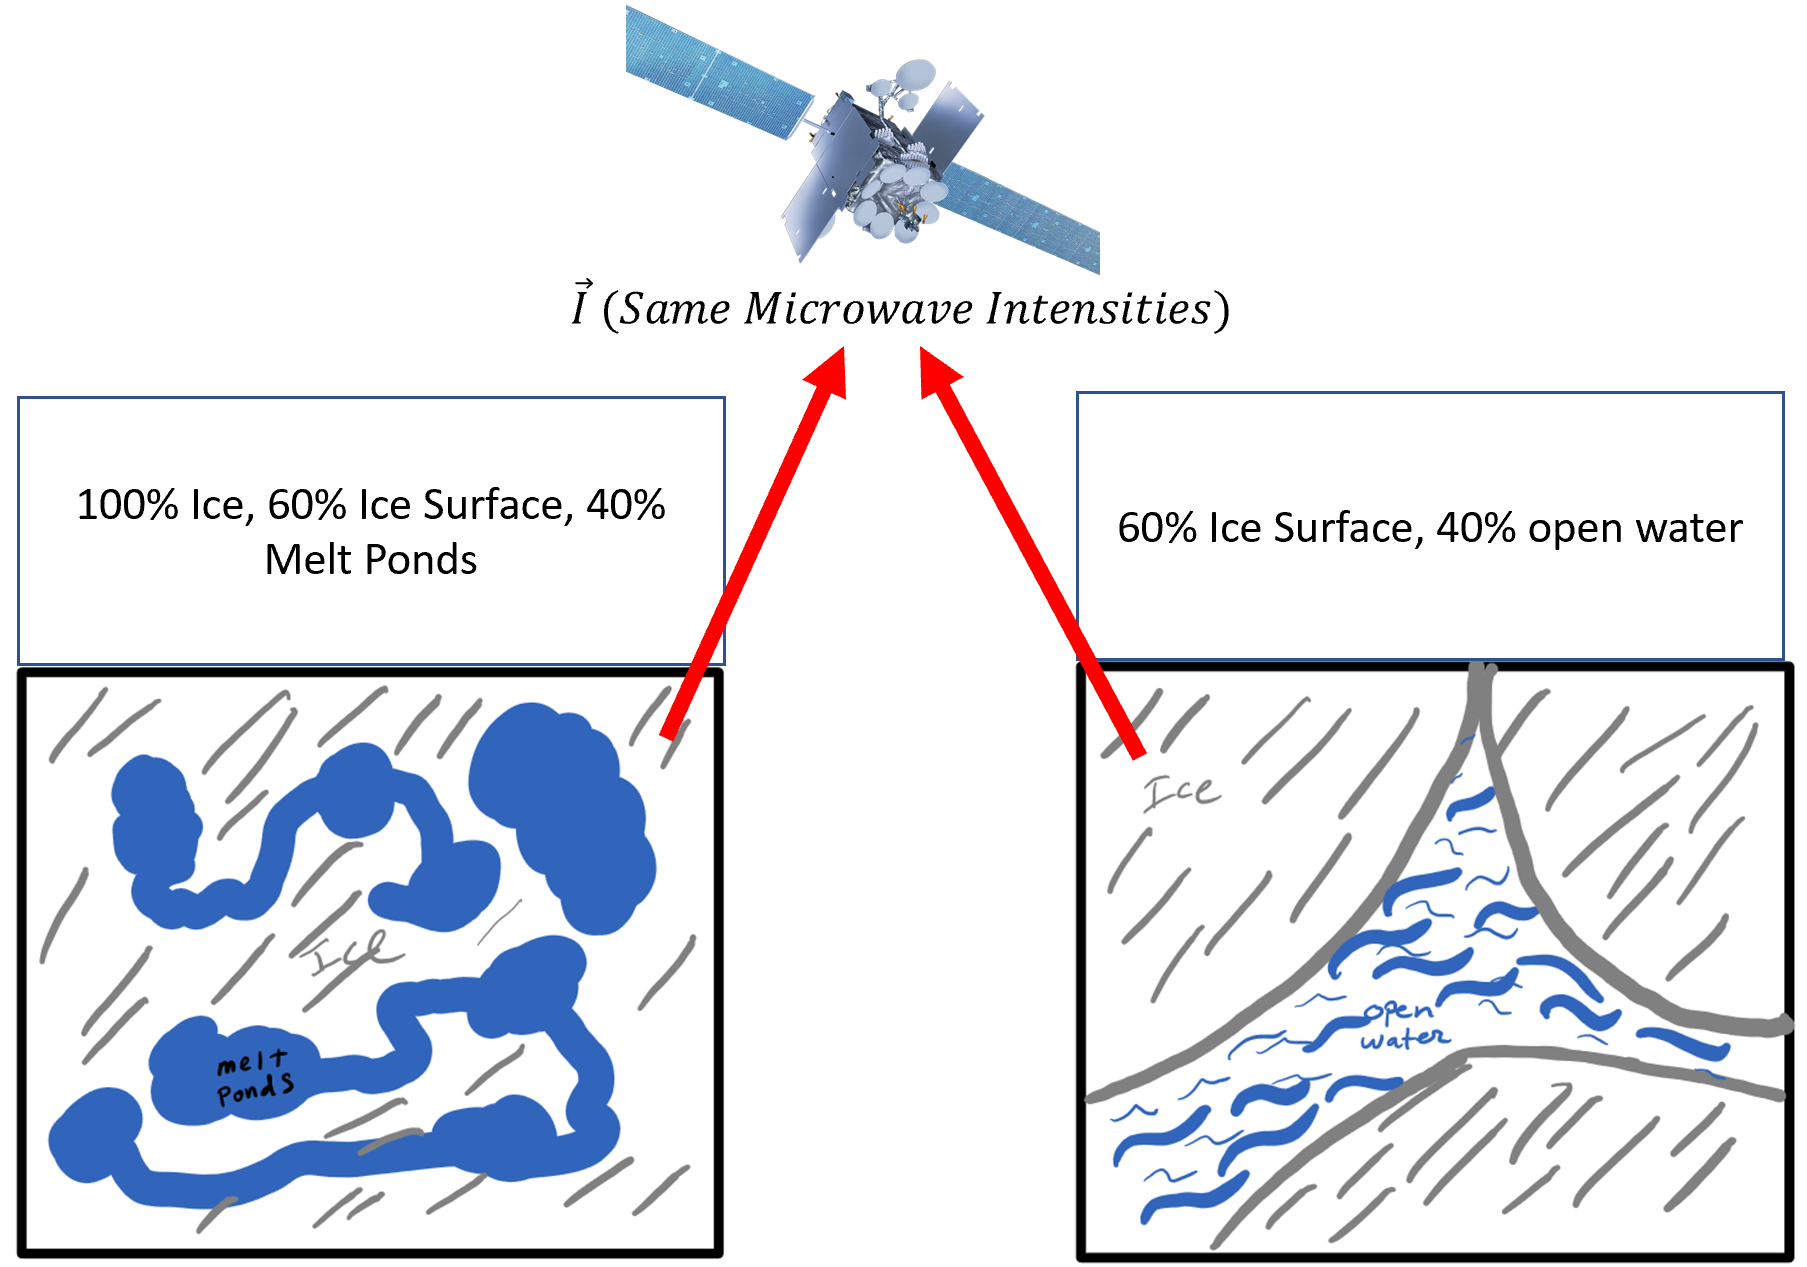
\includegraphics[width=\linewidth]{theylookthesame.PNG}
This can adversely affect sea ice forecasts when this incorrect data is assimilated. To improve the assimilation of this data, we propose to develop an observation operator which takes the model state directly to the satellite radiances avoiding the assimilation of incorrect values. This operator is difficult to model, computationally expensive, and depends on many parameters not included in current sea ice models. To circumvent this, we propose to machine learn this operator based on currently used sea ice state variables. As a first step, we study a simplified system based on a modified version of the sea ice energy balance model presented in (Eisenmann \& Wettlaufer 2009). This modified system is Filippov and produces data which mimics that of ice and observable satellite radiances under ponded conditions. We will present our results using learned observation operators for this proxy system and discuss how to extend the methodology to large scale models.


\end{multicols}

%\begin{multicols*}{2}
%\begin{vwcol}[widths={0.6,0.4}]

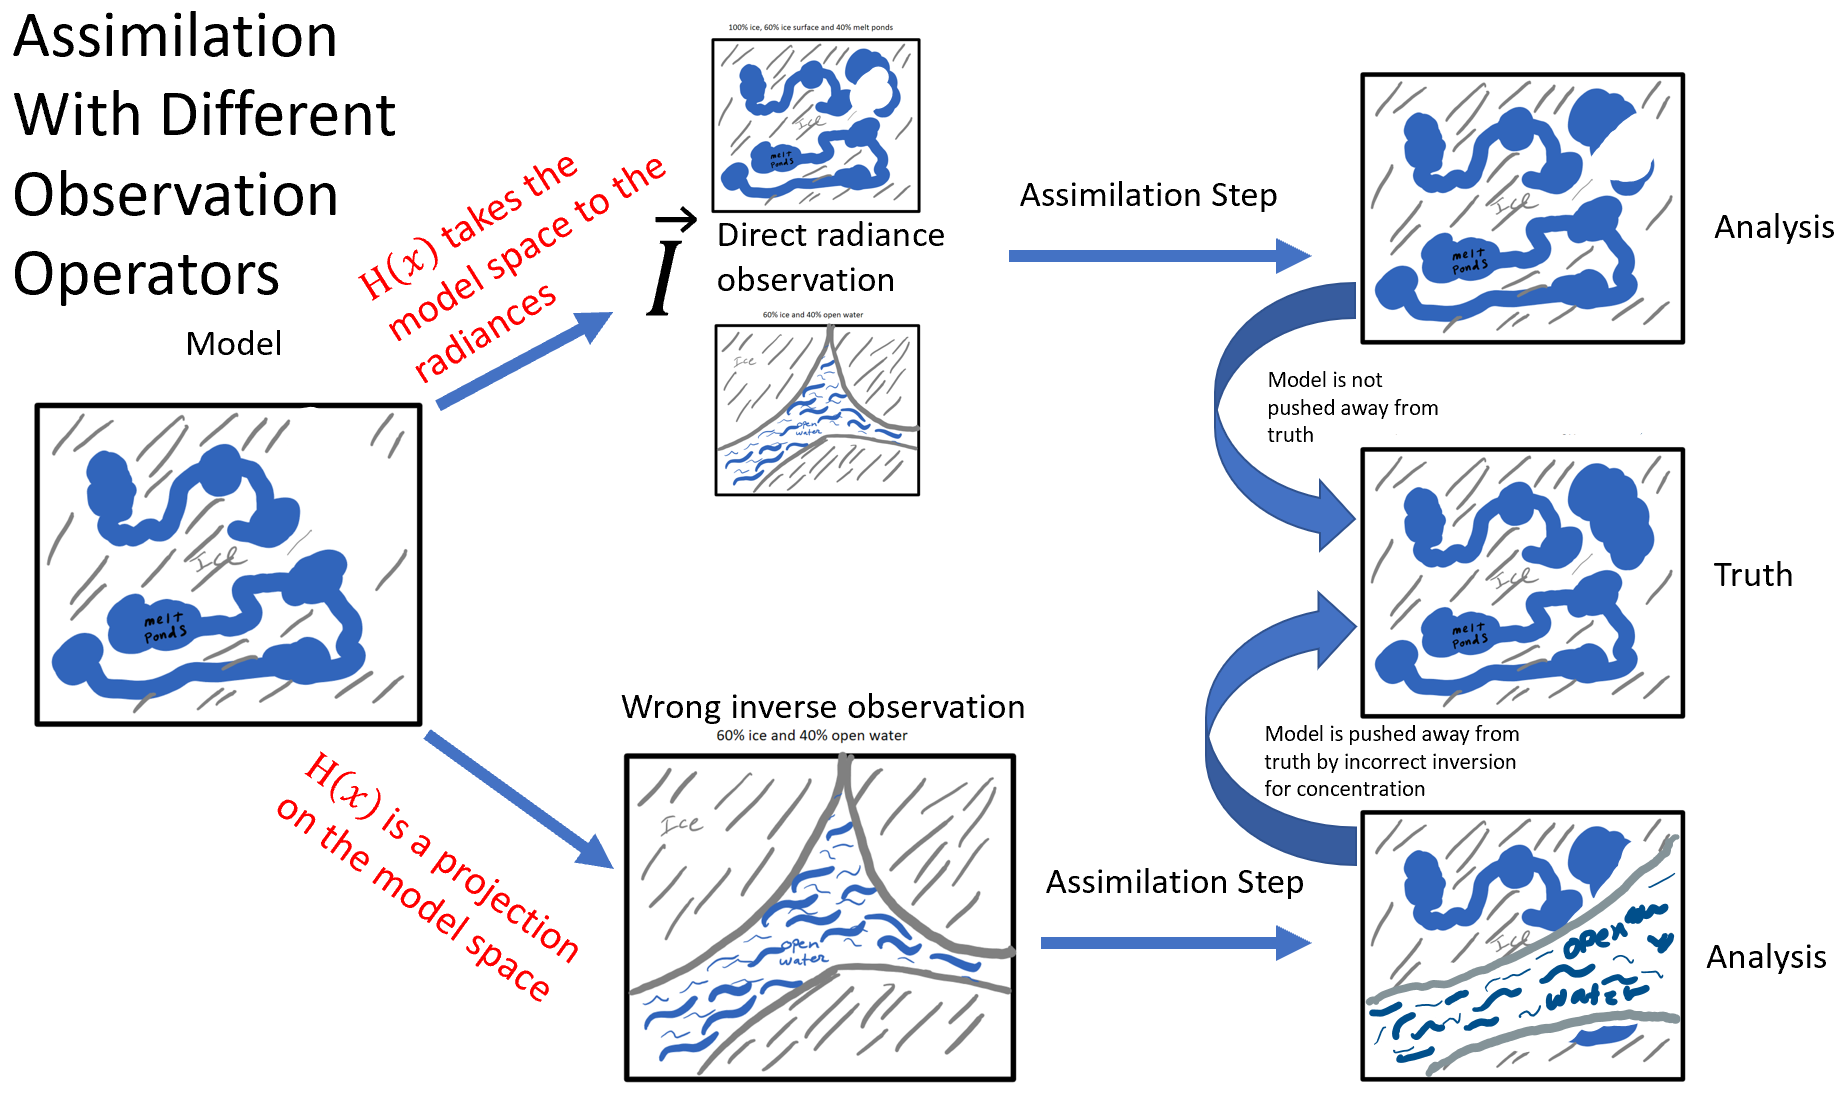
\includegraphics[width=\linewidth]{DAissues.PNG}


%\end{vwcol}
%\end{multicols*}



\vspace{0.3em} % When there are two boxes, some whitespace may need to be added if the one on the right has more content
}

%----------------------------------------------------------------------------------------
%	EnKF
%----------------------------------------------------------------------------------------

\headerbox{Ensemble Kalman Filter (EnKF)}{name=EnKF,column=0,span=2,below=intro,above=bottom}{ % This block's bottom aligns with the bottom of the conclusion block
\begin{multicols}{2}
The EnKF uses several model runs stemming from perturbed initial conditions to estimate the Error covariance matrices of the state vaiables and associated observations. These matrices in turn define the Kalman Gain ($K$) which is used to update each ensemble member.

\begin{enumerate}\compresslist
	\item Prediction step: $\mx_{t+1}^f=\cM(\mx_t^a)$ \\ 			$\mx^f$: the forecast
	\item Update step: $\mx^a=\mx^f + \mK(\my - \cH(\mx^f))$\\         $\mK$: Kalman gain matrix \\
			$\mx^a$: the analysis
	\item Repeat the steps.
\end{enumerate}
\end{multicols}
\centering{
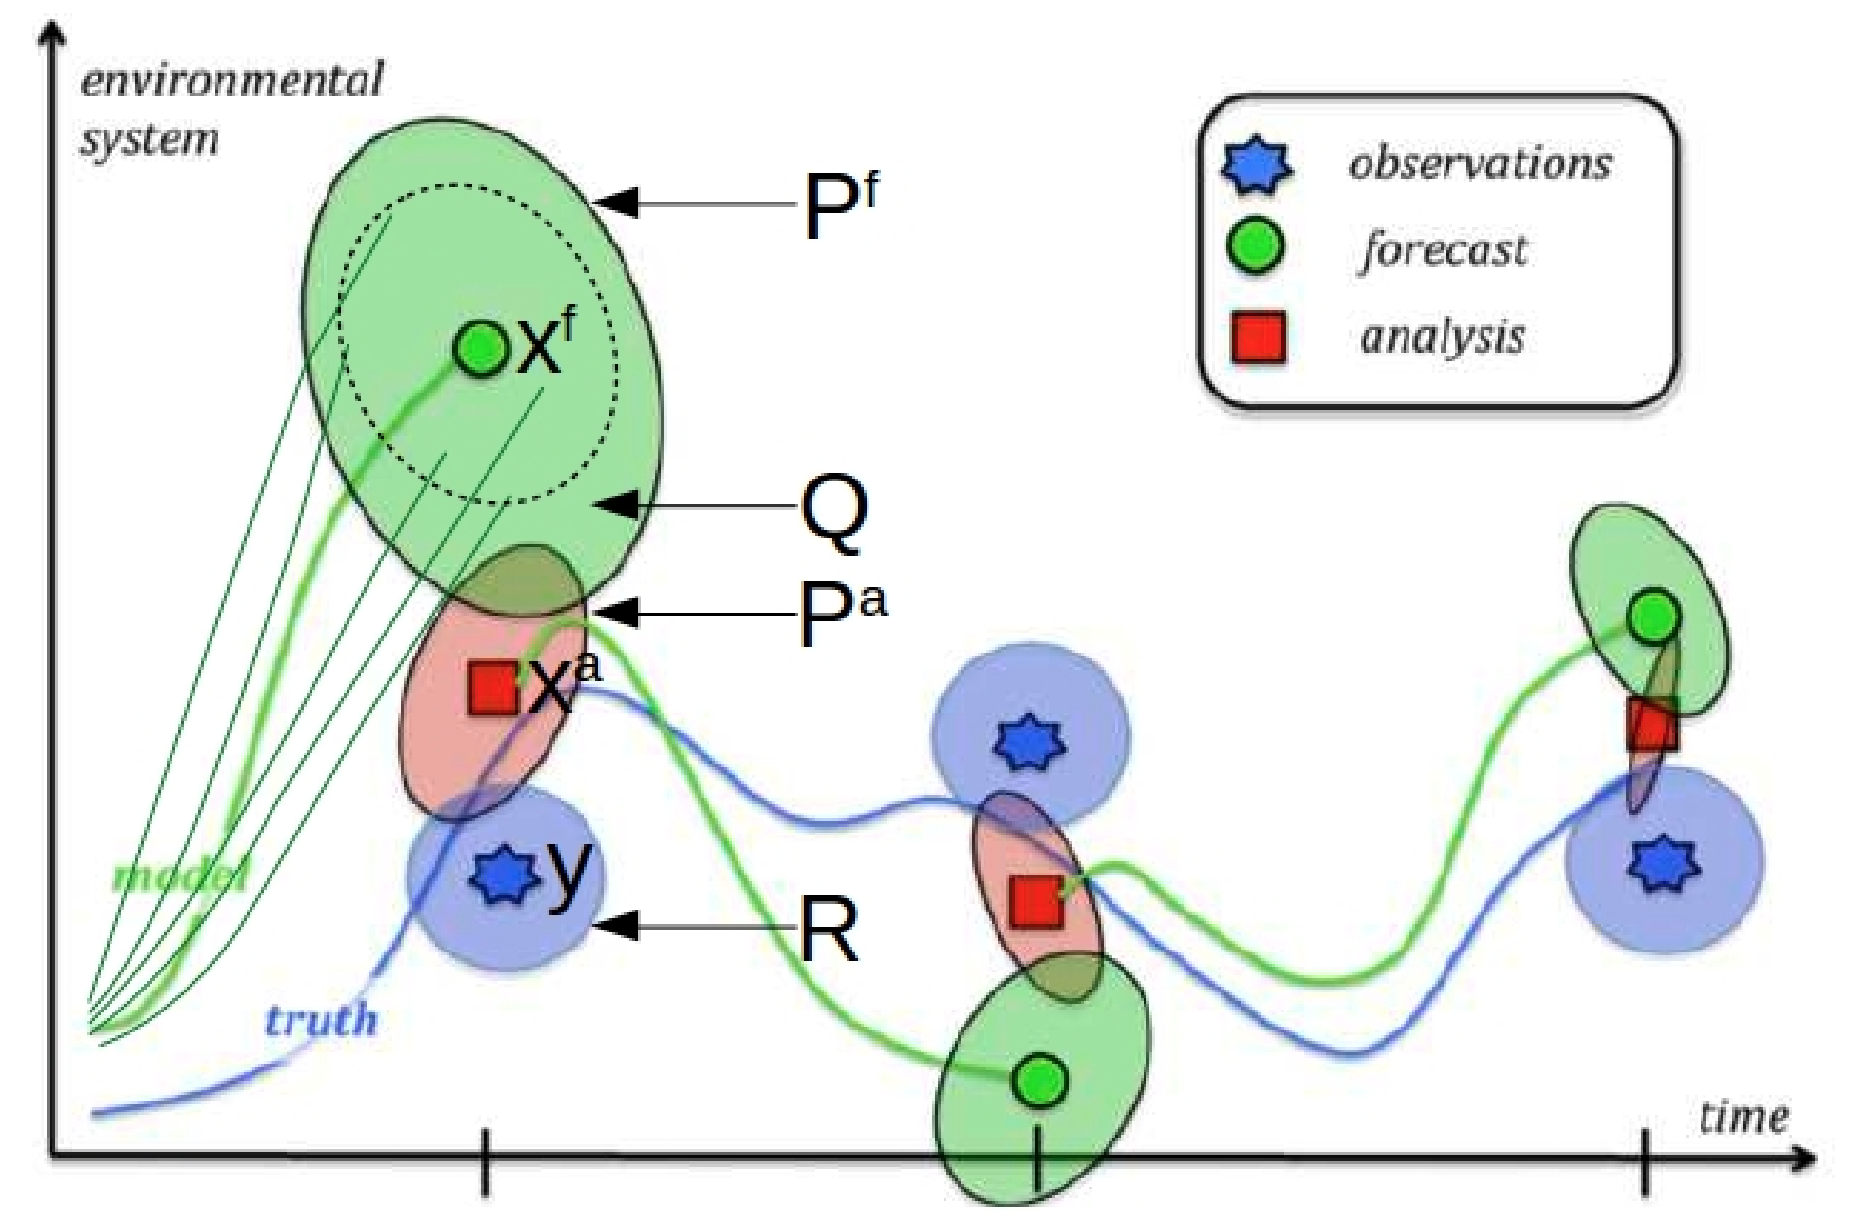
\includegraphics[width=.7\linewidth]{DAVisualization.png}
}

}

%----------------------------------------------------------------------------------------
%	Proxy Model
%----------------------------------------------------------------------------------------

\headerbox{Proxy Model}{name=model,column=2,row=0,span=2}{
\small{

\begin{multicols}{2}
In order to investigate the performance of a machine learned observation operator we have chosen to use a modified energy balance model based off of the one developed in (Eisenmann Wettlaufer 2009). We introduce a second varuable to this model, $\alpha_m$, the maximum attainable albedo. This variable provides information about the ``pond fraction" on top of the ice. When the energy variable $E$ is such that there is ice present, a lower value of $\alpha_m$ relates to the presence of melt ponds. The evolution of this variable is designed to mimic the fact that melt ponds initially form atop the ice, lowering albedo, and then drain into the ocean when the ice becomes permeable enough which leads to an increase in albedo. The evolution of $\alpha_m$ is taken to be driven by a competition of logistic terms, which depend on $E$. This is done is such a way that when we are in a very cold state $\alpha_m$ is driven to a value of $0.8$ representing snow covered ice. As the ice warms and $E$ increases $alpha_m$ is instead driven to $0.6$, the abledo of bare ice. When the albedo reaches $0.6$, the dynamics around $\alpha_m$ change such that when the energy is still negative and away from $E=0$, $alpha_m$ is driven lower toward $0.2$, the albedo of open water, to mimic pond formation. However when the energy approaches zero $\alpha_m$ is driven back toward $0.6$ to mimic pond drainage. From there, at positive energy values away from $E=0$ the albedo is driven again toward $0.2$ to mimic the melting of ice. The dynamics change when the system crosses the Fillipov curve defined by $H(E,\alpha_m)=\alpha(E,\alpha_m)-0.6=0$.



State model:
\begin{align*}\compresslist
&\frac{dE}{dt}=[1-\alpha(E,\alpha_{m})]F_s(t)-F_0(t)+F_{co_2}&\nonumber \\&-F_T(t)\frac{E}{c_{ml} H_{ml}}+F_B &\nonumber \\
&\frac{d \alpha_{m}}{dt}= \frac{E^2}{K_1^2}\alpha_{m}\left(1-\frac{\alpha_{m}}{0.8}\right) + \frac{K_2^2}{1+E^2}\alpha_{m}\left(1-\frac{\alpha_{m}}{0.6}\right) &\nonumber \\
&\quad\quad\quad\quad \textrm{in}  \quad S_1=\{(E,\alpha_m): H(E,\alpha_m)>0\} & \\
&\frac{ d \alpha_{m}}{dt}=\frac{K_3^2}{1+E^2}\alpha_{m}\left(1-\frac{\alpha_{m}}{0.6}\right) +\frac{E^2}{K_4^2}\alpha_{m}\left(1-\frac{\alpha_{m}}{0.2}\right) &\nonumber \\
&\quad\quad\quad\quad \textrm{in}  \quad S_2=\{(E,\alpha_m): H(E,\alpha_m)<0\}& \\
&\quad\quad\quad\quad \textrm{where} \quad H(E,\alpha_m)=\alpha(E,\alpha_m)-0.6.
\end{align*}
\end{multicols}

Using the state variables, we choose functions which give ice concentration $C_i$, pond concentration $C_p$, and a proxy for an inverted ice concentration $C_{sat}$ which cannot distinguish between open water and melt ponds. We also choose non injective functions to represent radiances based on the state variables.  

\begin{multicols}{2}
Proxy for concentration:\\
\begin{align*}\compresslist
C_i = &1-\left(\frac{0.8-\frac{1}{2}\left( \alpha_m+\alpha(E,\alpha_m)\right)}{0.6}\right) \\
C_p = &(0.5\tanh(\frac{E+200}{10})+0.5)\\
   & (1-\frac{0.2}{\alpha(E,\am)})^{1000}(1-\frac{\am}{0.8}) \\
\csat = &\max(0,C_i(E,\am)-C_p(E,\am))
\end{align*}
\vfill\null
\columnbreak
Proxy for observations:\\
\begin{equation*}
\begingroup
\renewcommand*{\arraystretch}{1.5}
\begin{bmatrix}
|E\alpha_m|\\ 
\alpha_m-\alpha(E,\alpha_m) \\
\alpha(E,\alpha_m)|E|\\
(0.5+0.4\tanh(\frac{50-E}{10}))(E+273.15)\\
C_i (1-\frac{\alpha(E,\alpha_m)}{\alpha_m})
\end{bmatrix}
\endgroup
\end{equation*}
\end{multicols}

\centering{
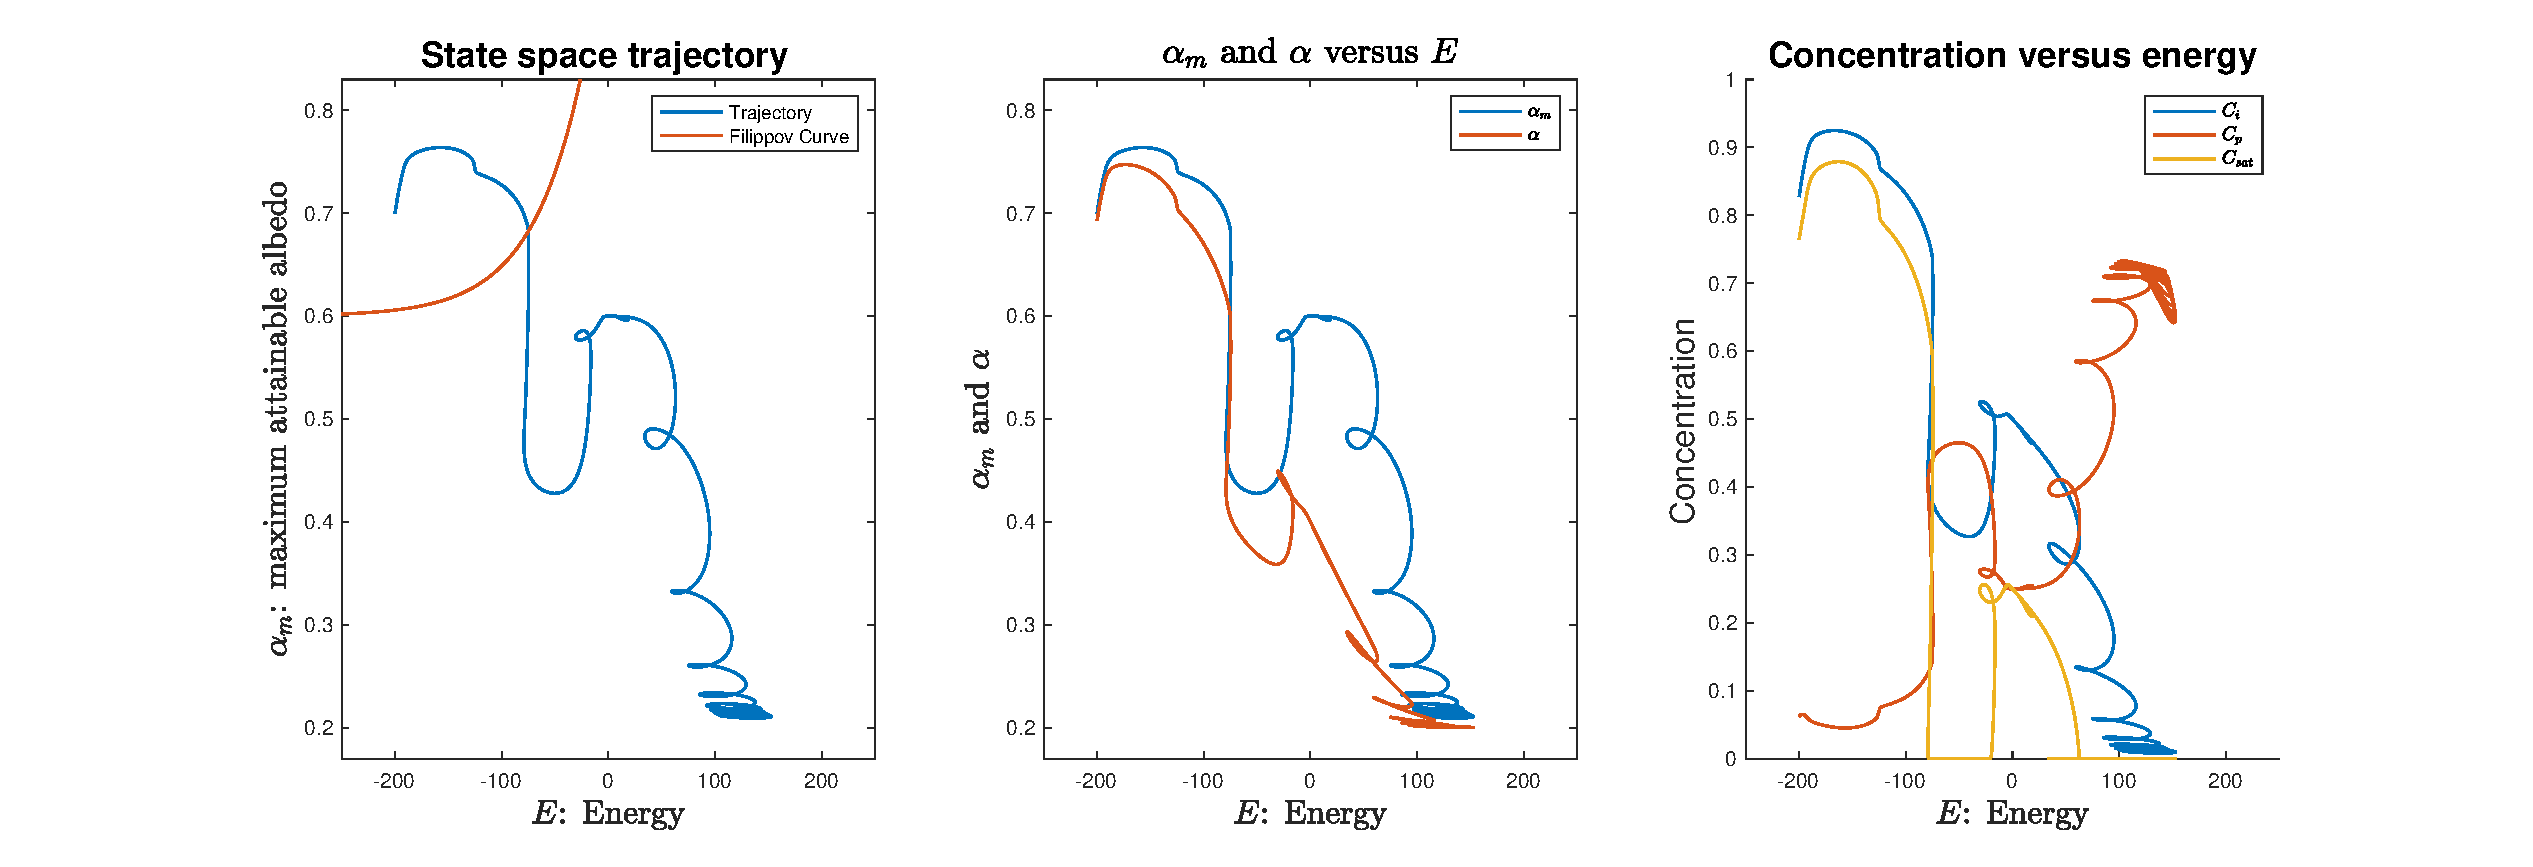
\includegraphics[width=\linewidth]{VersusEnergy.eps}
\captionof{figure}{Overview of the proposed proxy.}}
}
}

%----------------------------------------------------------------------------------------
%	Learning the Operator
%----------------------------------------------------------------------------------------

\headerbox{Learning the Operator}{name=learning,column=2,span=2,below=model,above=bottom}{
After experiments, we choose four layers to get our architecture shown below. The machine learning model can be written as a composed function.

\begin{equation*}
\scriptsize
\vy = \vx_{\text{out}} = \vW_4(\tanh(\vW_3(\tanh(\vW_2(\tanh(\vW_1 \vx_{\text{in}} + \vb_1))+\vb_2))+\vb_3))+\vb_4
\end{equation*}
$\vW_2,\vW_3,\vW_4$ are $5\times 5$ matrices, $\vW_1$ is a $5\times 2$ matrix and $\vb_1,\vb_2,\vb_3,\vb_4$ are $5$-dimensional vectors. The total number of parameters is $105$. The parameters are determined by the optimization algorithm.

\begin{center}
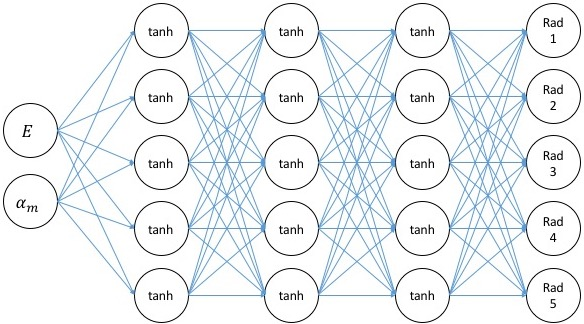
\includegraphics[width=.55\linewidth]{FNN.jpeg}
\end{center}
}

%----------------------------------------------------------------------------------------
%	Data Density
%----------------------------------------------------------------------------------------

\headerbox{Data Density}{name=density,column=4,span=3,row=0}{

\begin{itemize}\compresslist
	\item For the equilibrium states, where sufficient training data exists, our model tends to perform quite well.
	\item For the transient state, where training data is extremely sparse, the prediction does not make much sense.
\end{itemize}
\begin{multicols}{2}
\centering
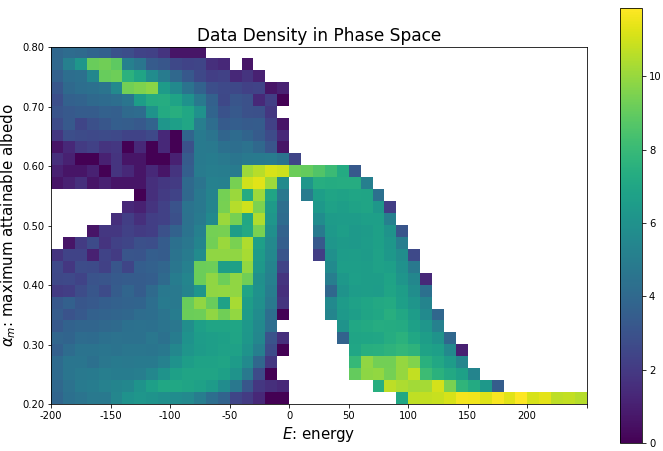
\includegraphics[width=.7\linewidth]{DensityMatrix.png}
\centering
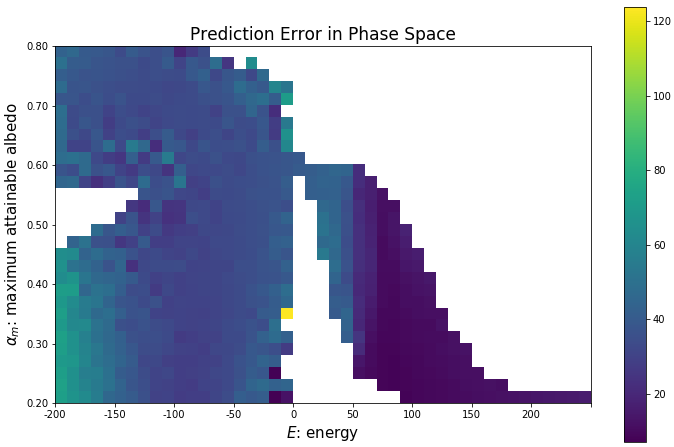
\includegraphics[width=.7\linewidth]{ErrorMatrix.png}
\end{multicols}

We address this issue in data assimilation with appropriate inflation.
\begin{multicols}{2}
The error covariance matrix for observation is estimated by the error in the machine learning algorithm $\mR_{i,i}(t) = \mxi_i(E(t),\am(t))$.
\vfill\null
\columnbreak
The inflation parameter is proportional to data density $\mP_t^a\rightarrow \mP_t^a+\frac{\mu\Lambda}{q}\mI_q$.
\end{multicols}

}

%----------------------------------------------------------------------------------------
%	Results
%----------------------------------------------------------------------------------------

\headerbox{Results}{name=results,column=4,span=3,below=density}{
%\begin{minipage}{0.5\linewidth}
%\centering{
%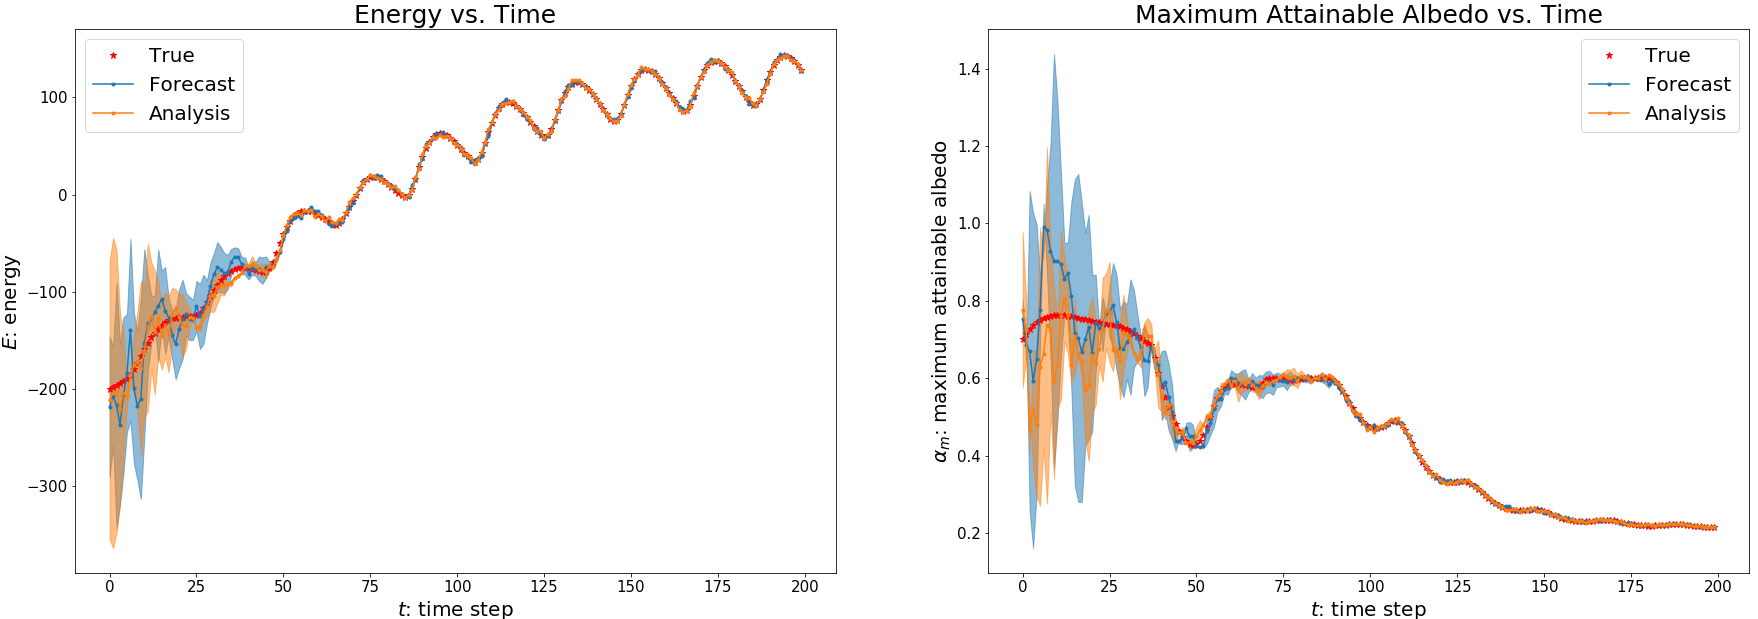
\includegraphics[width=\linewidth]{H_ml_hat_new.png}
%\captionof{figure}{DA with machine learning operator at radiance space}
%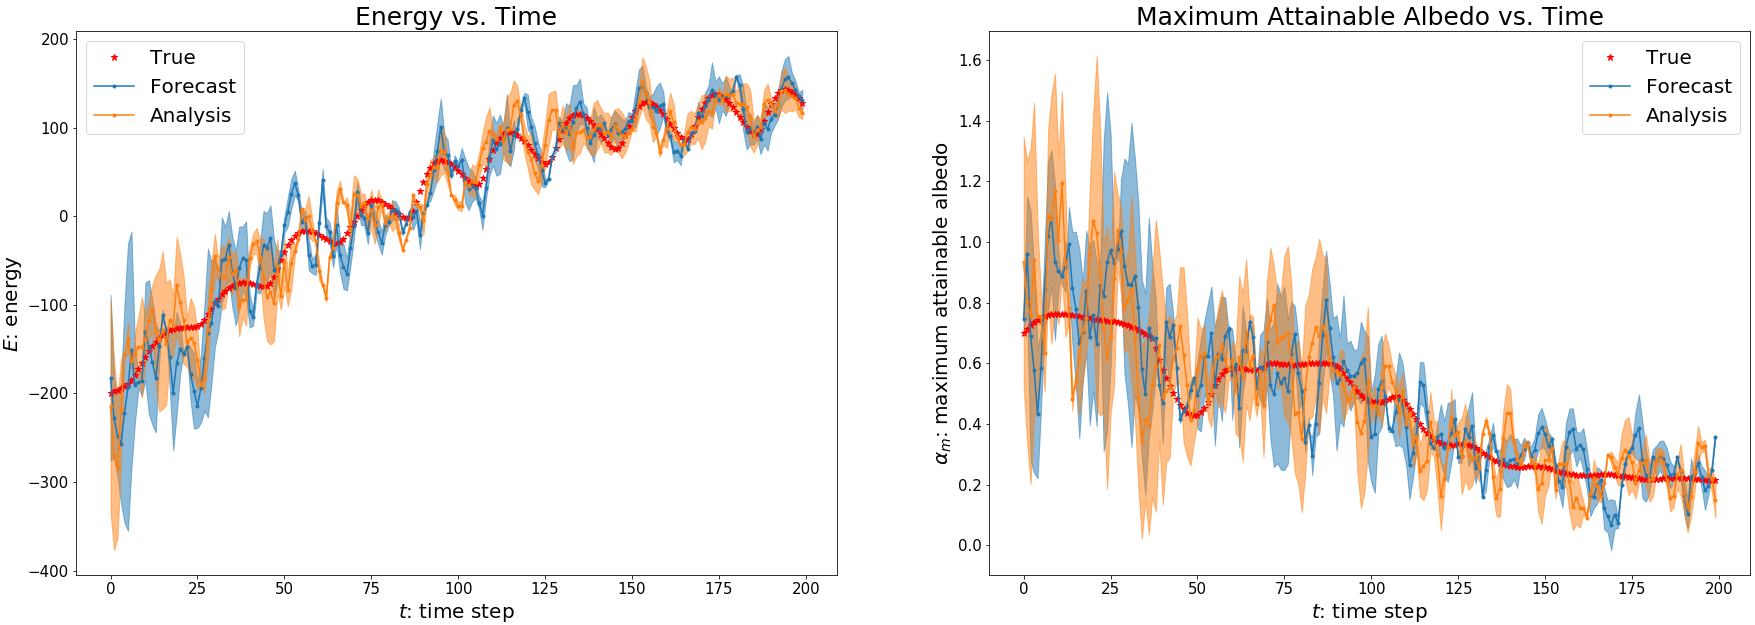
\includegraphics[width=\linewidth]{H_retrieval_new.png}
%\captionof{figure}{DA with retrieval algorithm at concentration space}
%}
%\end{minipage}

%\begin{multicols*}{2}
\centering
{\bf {\large Using the observation operator $H(E,\alpha_m)=C_i$.}}
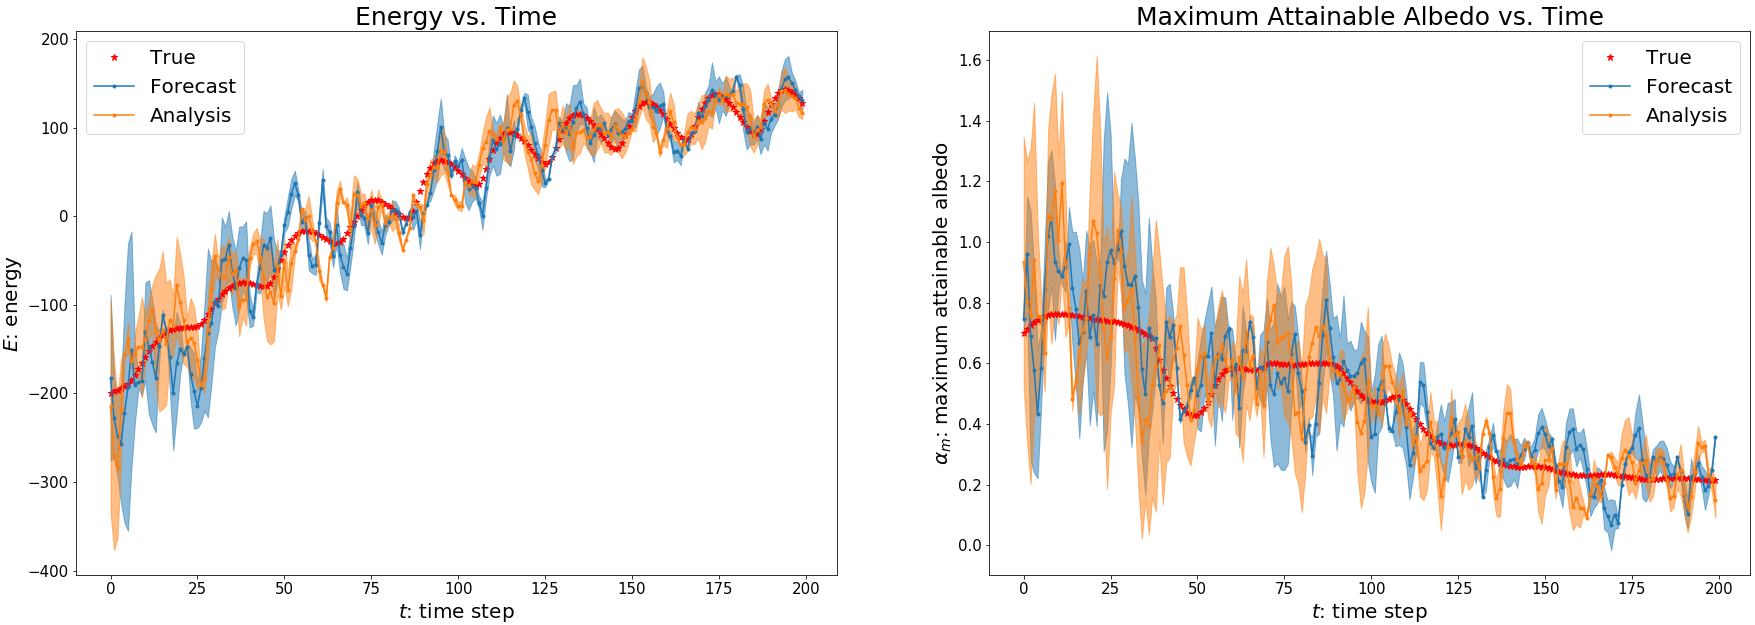
\includegraphics[width=.8\linewidth]{H_retrieval_new.png}
\

{\bf { \large Using the machine learned observation operator $H(E,\alpha_m)=[R_1,R_2,R_3,R_4,R_5]$.}}
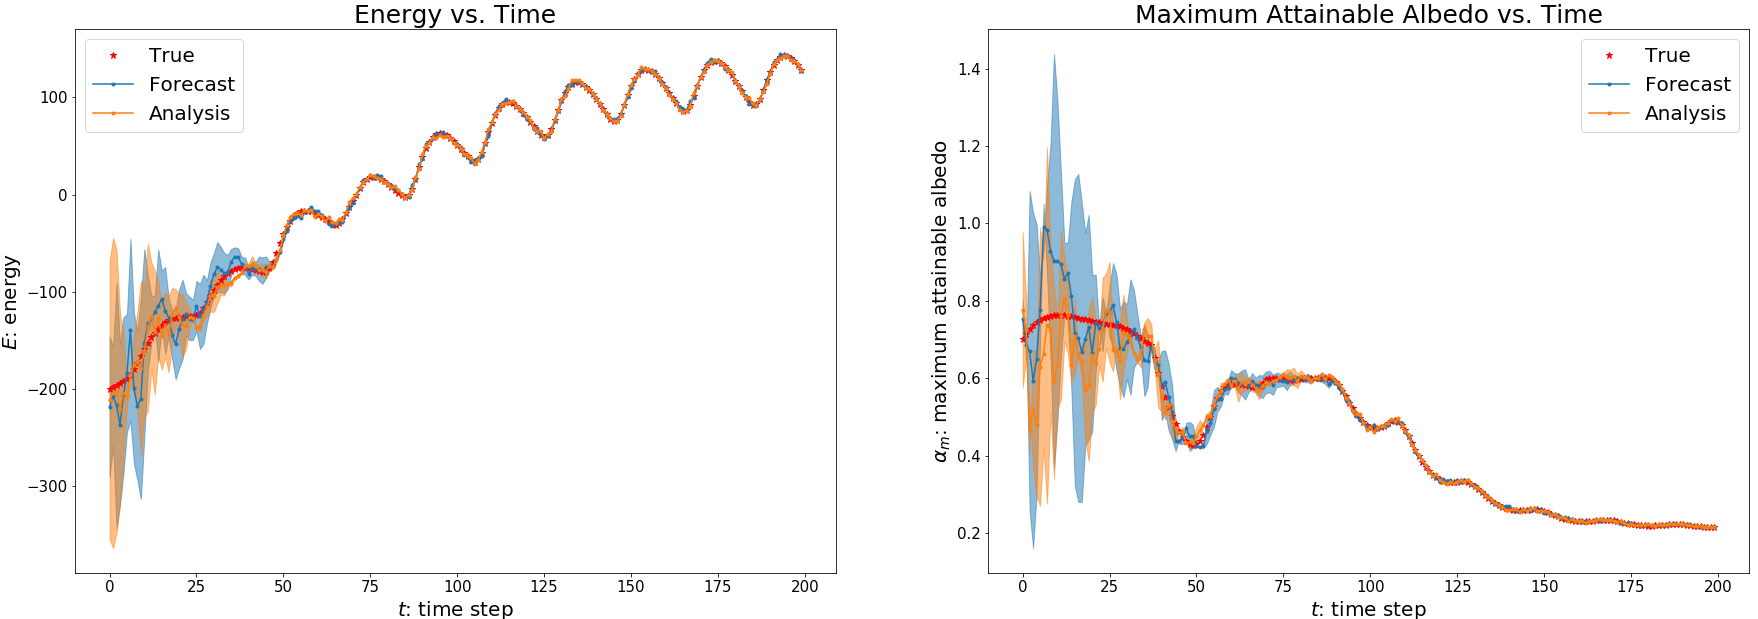
\includegraphics[width=.8\linewidth]{H_ml_hat_new.png}



%\end{multicols*}


% \begin{multicols}{2}

% \tikzstyle{decision} = [diamond, draw, fill=blue!20, text width=4.5em, text badly centered, node distance=2cm, inner sep=0pt]
% \tikzstyle{block} = [rectangle, draw, fill=blue!20, text width=5em, text centered, rounded corners, minimum height=4em]
% \tikzstyle{line} = [draw, -latex']
% \tikzstyle{cloud} = [draw, ellipse, fill=red!20, node distance=3cm, minimum height=2em]

% \begin{tikzpicture}[node distance = 2cm, auto]
% \node [block] (init) {Initialize Model};
% \node [cloud, left of=init] (Start) {Start};
% \node [cloud, right of=init] (Start2) {Start Two};
% \node [block, below of=init] (init2) {Initialize Two};
% \node [decision, below of=init2] (End) {End};
% \path [line] (init) -- (init2);
% \path [line] (init2) -- (End);
% \path [line, dashed] (Start) -- (init);
% \path [line, dashed] (Start2) -- (init);
% \path [line, dashed] (Start2) |- (init2);
% \end{tikzpicture}

% %------------------------------------------------

% \begin{itemize}\compresslist
% \item Pellentesque eget orci eros. Fusce ultricies, tellus et pellentesque fringilla, ante massa luctus libero, quis tristique purus urna nec nibh. Phasellus fermentum rutrum elementum. Nam quis justo lectus.
% \item Vestibulum sem ante, hendrerit a gravida ac, blandit quis magna.
% \item Donec sem metus, facilisis at condimentum eget, vehicula ut massa. Morbi consequat, diam sed convallis tincidunt, arcu nunc.
% \item Nunc at convallis urna. isus ante. Pellentesque condimentum dui. Etiam sagittis purus non tellus tempor volutpat. Donec et dui non massa tristique adipiscing.
% \end{itemize}

% \end{multicols}
}

%----------------------------------------------------------------------------------------
%	Conclusion & Furture Direction
%----------------------------------------------------------------------------------------

\headerbox{Conclusions and Future Directions}{name=conclusion,column=4,span=3,below=results,above=bottom}{
%In conclusion, for data assimilation in sea ice concentration with melt ponds, it is a desirable option to use historic data to construct a machine learning observation operator taking the state variables directly to the satellite radiances. Even if only a small amount of historic data is available for training or the data is highly noisy, machine learning is still likely to offer a better solution than satellite retrieval algorithm.

%\par We will try using other machine learning algorithms like XGBoost and Random Forest. The particle filter is a reasonable choice to do data assimilation with.
%\par We will test our idea on larger scale models that are actually used in the reality, e.g. The Community Sea Ice Model CICE along with an atmospheric radiative transfer model.
%\par The eventual goal of our study is to build a machine learning model that takes sea ice states to the satellite radiances.

The observation operator is a critical part of any data assimilation scheme. In the case where inversion of state variables from observations are difficult, and direct calculation of observations from state variables are too expensive or difficult, the observation operator can be learned form available data. Machine learned observation operators also have the advantage of automatically parameterizing possibly unknown relationships between state variables and observed values. This of courses depends on the quality and availability of data. For this simple model case we have demonstrated this principle and explored how error in the learned operator may affect the analysis step. 

\vspace{.1cm} Our ultimate goal will be to apply these ideas to a large scale numerical sea ice model. The data set available for training an observation is mostly limited to instances where passive microwave measurements can be matched to optical images of sea ice. A primary challenge of training a suitable operator will be the estimation of sea ice state variables form the images. This will produce error in the data set itself. For this purpose we will also employ the use of a radiative transfer model which we can use to simulate observed satellite radiances from known sea ice state variables to augment our data set. We anticipate also using atmospheric information as input to the operator. We will also test several methods for learning the operator and evaluate the performance of each. 

}

%----------------------------------------------------------------------------------------

\end{poster}

\end{document}